\newpage
\hypertarget{remCard tex}{}
\subsection{Implementing removeCard}
\texHeader

\begin{itemize}

\item[$\blacktriangleright$] Open \texttt{Partition.eclass}, go to the \texttt{removeCard} signature and add a pair of curly brackets so that it looks like a
proper method declaration. This entire scope can be referred to as the method's \emph{activity}, where the control flow (imperative top-layer) of a
transformation is defined.

\item[$\blacktriangleright$] Complete the activity with a single pattern and return statement as depicted in Fig~\ref{eclipse:remCardDec}. Don't forget -- you
can use eMoflon's auto-complete feature here! Press \texttt{Ctrl + Space} on an
empty line, then select the pattern template to establish \texttt{deleteSingleCard}.

\item[$\blacktriangleright$] Note that in this context, the \texttt{`@'} operator indicates an \emph{ObjectVariableExpression}%
\define{ObjectVariable\-Expression}. This expression implicitly refers to object variables from the preceding story node. In \texttt{removeCard}'s case, the
returned object refers to the \texttt{card} from the pattern.

\vspace{0.5cm}

\begin{figure}[htp]
\begin{center}
  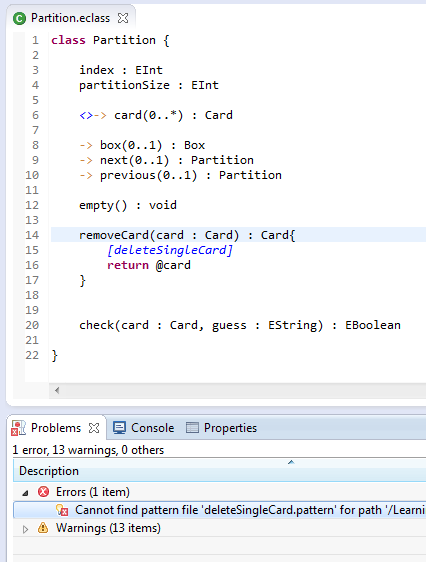
\includegraphics[width=0.5\textwidth]{eclipse_removeCardDeclaration}
  \caption{Control flow for \texttt{removeCard}}
  \label{eclipse:remCardDec}
\end{center}
\end{figure}

\item[$\blacktriangleright$] It should be mentioned that MOSL limits method definitions exclusively to the method's control flow. All actual transformation
rules are modeled in separate \emph{pattern} files. In this case, \texttt{removeCard}'s link deletion will be modeled in \texttt{[deleteSingleCard]}.

\vspace{0.5cm}

\item[$\blacktriangleright$] Save \texttt{Partition.eclass}. An error should immediately appear below the editor. In the ``Problems'' tab, the message
states that the builder cannot find the specified pattern file. Well, this makes sense. You haven't created it yet! Click this message and press \texttt{Ctrl +
1} to invoke a ``Quick Fix'' dialogue (Fig~\ref{eclipse:quickFix}). It offers to create a pattern file for you. Given that's exactly what you'd like, select the
option and press \texttt{Finish}.

\vspace{0.5cm}

\begin{figure}[htp]
\begin{center}
  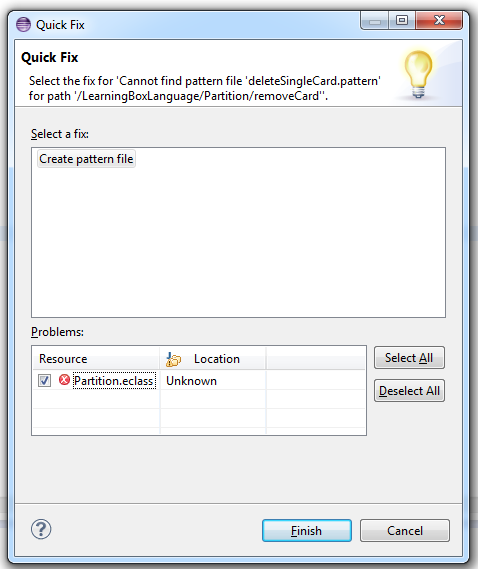
\includegraphics[width=0.5\textwidth]{eclipse_patternQuickFix}
  \caption{A quick fix to a missing pattern error}
  \label{eclipse:quickFix}
\end{center}
\end{figure}

\item[$\blacktriangleright$] The new file will open in the editor, and you'll be able to see a new directory structure under ``LearningBoxLanguage/\_patterns''
(Fig.~\ref{eclipse:pattStruct}). To explain, \texttt{deleteSingleCard.pattern} is invoked by the method \texttt{removeCard}, which is in the \texttt{Partition}
EClass. \texttt{Partition} will eventually contain a folder for each method that uses a pattern.

\vspace{0.5cm}

\item[$\blacktriangleright$] The content of any pattern file is simply a list \emph{object variable scopes}, and then,
within such a scope, operations such as `delete/create/find' this outgoing reference. Remember - the main goal of SDMs is to focus here is not on \emph{how},
but \emph{what}.

\newpage

\begin{figure}[htp]
\begin{center}
  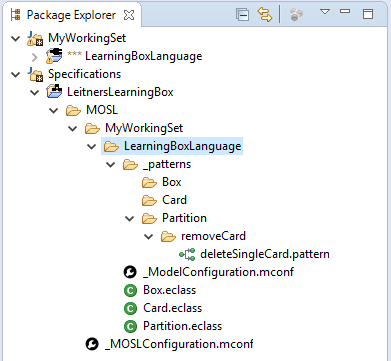
\includegraphics[width=0.9\textwidth]{eclipse_patternStructure}
  \caption{Directory structure for a pattern}
  \label{eclipse:pattStruct}
\end{center}
\end{figure}

\item[$\blacktriangleright$] Create two object variables, \texttt{@this:Partition } and \texttt{ @card:Card}\\ (Fig.~\ref{eclipse:remCardObjVar}). When working
with MOSL patterns, \texttt{`@'} again indicates that the variable is \emph{bound}. \texttt{this} is bound to the object whose method is invoked,
while \texttt{card} is bound to the value of the parameter with the same name.

\begin{figure}[htp]
\begin{center}
  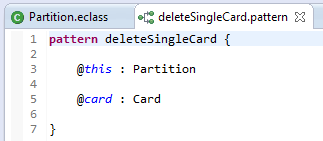
\includegraphics[width=0.6\textwidth]{eclipse_thisObjVar}
  \caption{Object variables for \texttt{removeCard}}
  \label{eclipse:remCardObjVar}
\end{center}
\end{figure}

\item[$\blacktriangleright$] Object variable scopes determine the changes to be applied to the any exiting references of the variable. Therefore, add:
\syntax{-- -> card:card} to \texttt{@this} to destroy the \texttt{card} reference targeting the \texttt{card} object. Your pattern should now resemble
Fig.~\ref{eclipse:deleteReference}. 

\begin{figure}[htp]
\begin{center}
    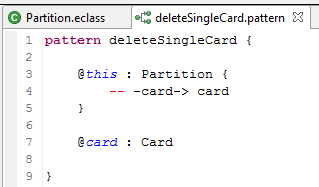
\includegraphics[width=0.6\textwidth]{eclipse_remCardObjVars}
  \caption{Destroy the link between a card and its partition}
  \label{eclipse:deleteReference}
\end{center}
\end{figure}
\newpage

\item[$\blacktriangleright$] In summary, any \emph{outgoing link variable}\define{Outgoing~Link Var\-i\-able} follows this syntax:

\syntax{[action]`->'nameOfOutgoingLV`:'targetOV\\
\\
With:\\
action := `--' | `++' | `!'\\
nameOfOutgoingLV := STRING\\
targetOV := STRING
}

\item[$\blacktriangleright$] If you ever need to quickly remind yourself of specific reference or attribute names, press \texttt{alt} and the \texttt{left}
arrow to jump back from your pattern to your EClass. Conversely, to quickly open
or jump to a pattern, hover over the pattern name while holding \texttt{Ctrl}
until it's underlined, then click!

\item[$\blacktriangleright$] Remember, links between classes can be specified as \emph{bidrectional EReferences},\footnote{Technically two
\emph{unidirectional EReferences}. Refer to Part II, Section 2.5.} linked together as opposites in ``LearningBoxLanguage/\_con\-straints.mconf.'' In this case,
therefore, we don't need to worry about declaring \texttt{-- -> cardContainer:Card} inside \texttt{card}, as it would be redundant.

\item[$\blacktriangleright$] Save and build your metamodel. If any errors occur, double check and make sure your activity and pattern match ours. 

\item[$\blacktriangleright$] To see how the same method is crafted in the visual syntax, check out Fig.~\ref{ea:sdm_complete_control_flow} from the previous
section.

\end{itemize}
